\chapter{Introduction} \label{chap:intro}

\section{Background: the ``death ray'' that saves lives}

Like many modern technologies such as computers, the internet, and GPS whose origins can be traced back to the military, aviation radar is no exception. 

The fundamental theory of radar started in late 19th century. Since the 1860s, when the electromagnetic theory was discovered by James Clerk Maxwell, the foundation for many science and technology fields was laid out. In the late 19th century, Heinrich Hertz, who proved the existence of electromagnetic waves, also confirmed that metals could reflect radio waves. In the first decades of the 20th century, several systems for using radio waves to provide short-range directional information of objects were developed. German inventor Christian Hulsmeyer is often considered as the first person to use radio waves to detect metal objects in 1904.

However, not until the Second World War, was the concept of \emph{RAdio Detection And Ranging} (RADAR) developed. The technology was simultaneously researched by both major Allies and Axis countries. However, the United Kingdom led the race to in developing a functional radar system. 

Originally, British Air Ministry officials, who were concerned about falling behind the technology race with the Germans, advised the physicist Robert Watson Watt to propose a set of abstract technical challenges to his colleague Skip Wilkins:

\begin{quotation}
\noindent"Suppose, just suppose, that you had eight pints [17kg] of water, 3,000ft [1km] above the ground. And suppose that water was at 98$^\circ$F [37$^\circ$C], and you wanted to heat it to 105$^\circ$F [41$^\circ$C]. How much radio frequency power would you require, from a distance of 5km?"
\end{quotation}

Both scientists understood very well that the average adult human has 17 kg blood and a critical body temperature of 41$^\circ$C. This represented an idea of the \emph{death ray} that could be used to disable enemy aircraft pilots.

Without even developing such a system, they figured out that the power requirement was far beyond practice at that time. However, they realized an opportunity for funding a different project. Given the amount of power that can be transmitted, it was possible to detect the reflection of aircraft, and, thus calculate the position of aircraft. This proposal was approved by the air ministry. Later on, this technology was developed and shared with Americans during the war. After that, the widespread usage of RADAR (later became radar) had begun.

After the war ended, radar became more and more important for civil aviation. With the rapid growth of commercial flights, it developed into a prominent technology for aircraft surveillance in the aviation industry.

\section{The primary radar}

Aircraft surveillance in the early days relied only on, what is known today as the primary surveillance radar (PSR). The concept of PSR is fairly simple. It is a rotating radio transponder with an omnidirectional antenna. Commonly, the radar transmits a one-microsecond pulse for every one millisecond and listens to the reflections from the airplanes. The position of the aircraft is measured by distance and angle to the radar. The distance is known as slant distance, which is the line-of-sight distance between an aircraft and the radar. It can be calculated by measuring the time difference between the original signal and the reflection received, since the speed of the radio wave (speed of light) is known. The azimuth angle\footnote{Azimuth angle is the horizontal angle measured clockwise with to the north of the observer.} of the aircraft is determined by the rotation angle of the radar. By processing radar signals, technologies like phase filter and Doppler filter can be used to filter out moving targets like aircraft and remove static objects, such as mountains, buildings, and other obstacles.

The slant distance of an aircraft does not always correspond to the horizontal distance to the radar. This is because all points having the same slant distance are located on a sphere that has the radius equal to the distance. Since the civil radar usually does not provide elevation information on the target, it is not possible to accurately convert the slant distance to the horizontal distance. Historically, it is sufficient to use primary radar for separating airplanes without considering this altitude differences. However, other systems have to be in place to provide air traffic controllers more accurate positions of the aircraft.

\section{The secondary radar}

The secondary surveillance radar (SSR), also known as air traffic control radar beacon system (ATCRBS), was designed to provide air traffic controllers more information than that provided by the primary radar. The secondary radar can be installed separately or installed on top of the primary radar. It uses a different radio frequency to actively interrogate the aircraft and receive information transmitted by the aircraft.

The SSR transmits interrogations using the 1030 MHz radio frequency and the aircraft transponder transmits replies using 1090MHz radio frequency. In the early design of SSR, two civilian communication protocols (Mode~A and Mode~C) were introduced. Mode~A and Mode~C allow the SSR to continuously interrogate the identity (squawk code) and the barometric altitude of an aircraft respectively.

Although Mode~A and Mode~C provide additional information to air traffic controllers, they present several design challenges \cite{icao1983}. The secondary surveillance radar initiates Mode~A and C interrogations with two different pulse patterns, which are shown in Figure \ref{fig:mode_ac_uplink_pulses}.

\begin{figure}[ht]
  \scalebox{0.9}{
    

\tikzset{every picture/.style={line width=0.75pt}} %set default line width to 0.75pt

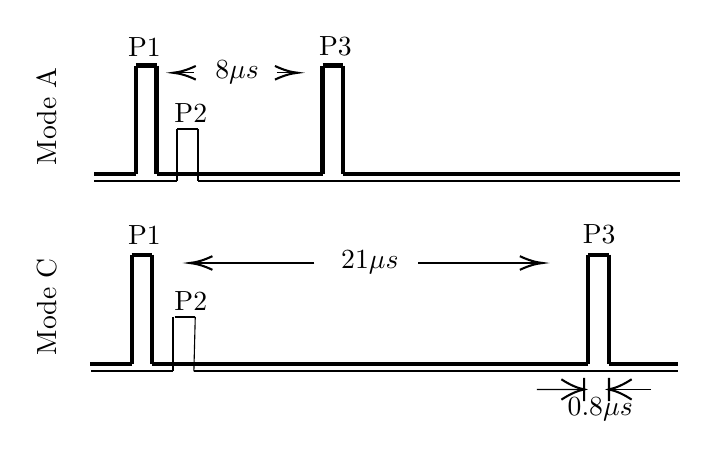
\begin{tikzpicture}[x=0.75pt,y=0.75pt,yscale=-1,xscale=1]
%uncomment if require: \path (0,311.79999923706055); %set diagram left start at 0, and has height of 311.79999923706055

%Straight Lines [id:da4787976488023191]
\draw [line width=1.5]    (47.72,77.93) -- (67.72,77.93) ;


%Straight Lines [id:da1666431573130951]
\draw [line width=1.5]    (67.72,25.72) -- (67.72,77.93) ;


%Straight Lines [id:da84341460830449]
\draw [line width=1.5]    (77.72,77.93) -- (157.72,77.93) ;


%Straight Lines [id:da9133073187219447]
\draw [line width=1.5]    (77.72,25.72) -- (77.72,77.93) ;


%Straight Lines [id:da3418906226920402]
\draw [line width=1.5]    (67.72,25.72) -- (77.72,25.72) ;


%Straight Lines [id:da7739092671946766]
\draw [line width=0.75]    (87.72,56.27) -- (87.72,81.41) ;


%Straight Lines [id:da40386604842800855]
\draw [line width=0.75]    (47.72,81.41) -- (87.72,81.41) ;


%Straight Lines [id:da004748895899417738]
\draw [line width=1.5]    (157.72,25.72) -- (157.72,77.93) ;


%Straight Lines [id:da23486773411516415]
\draw [line width=1.5]    (167.72,25.72) -- (167.72,77.93) ;


%Straight Lines [id:da8236386700565863]
\draw [line width=1.5]    (157.72,25.72) -- (167.72,25.72) ;


%Straight Lines [id:da9092733889117579]
\draw [line width=1.5]    (167.72,77.93) -- (330,77.93) ;


%Straight Lines [id:da5605933319835226]
\draw    (97.72,56.27) -- (97.72,81.41) ;


%Straight Lines [id:da7141828320776771]
\draw [line width=0.75]    (87.72,56.27) -- (97.72,56.27) ;


%Straight Lines [id:da3052256663595232]
\draw [line width=0.75]    (97.72,81.41) -- (330,81.41) ;


%Straight Lines [id:da40305669598670657]
\draw    (135.72,29.2) -- (143.72,29.2) ;
\draw [shift={(145.72,29.2)}, rotate = 180] [color={rgb, 255:red, 0; green, 0; blue, 0 }  ][line width=0.75]    (10.93,-3.29) .. controls (6.95,-1.4) and (3.31,-0.3) .. (0,0) .. controls (3.31,0.3) and (6.95,1.4) .. (10.93,3.29)   ;

%Straight Lines [id:da546905475224932]
\draw    (95.72,29.2) -- (87.72,29.2) ;
\draw [shift={(85.72,29.2)}, rotate = 360] [color={rgb, 255:red, 0; green, 0; blue, 0 }  ][line width=0.75]    (10.93,-3.29) .. controls (6.95,-1.4) and (3.31,-0.3) .. (0,0) .. controls (3.31,0.3) and (6.95,1.4) .. (10.93,3.29)   ;

%Straight Lines [id:da9766240369140216]
\draw [line width=1.5]    (45.72,169.58) -- (65.72,169.58) ;


%Straight Lines [id:da59866225699548]
\draw [line width=1.5]    (65.72,116.79) -- (65.72,169.58) ;


%Straight Lines [id:da008830950143269067]
\draw [line width=1.5]    (75.72,169.58) -- (285.72,169.58) ;


%Straight Lines [id:da15080830342823326]
\draw [line width=1.5]    (75.72,116.79) -- (75.72,169.58) ;


%Straight Lines [id:da23329569370383663]
\draw [line width=1.5]    (65.72,116.79) -- (75.72,116.79) ;


%Straight Lines [id:da88960254128125]
\draw [line width=0.75]    (85.72,146.76) -- (85.72,173.06) ;


%Straight Lines [id:da15138888301724762]
\draw [line width=0.75]    (46.39,173.06) -- (85.72,173.06) ;


%Straight Lines [id:da8091412830946654]
\draw [line width=1.5]    (285.72,116.79) -- (285.72,169.58) ;


%Straight Lines [id:da4944822301415428]
\draw [line width=1.5]    (295.72,116.79) -- (295.72,169.58) ;


%Straight Lines [id:da7980939736484842]
\draw [line width=1.5]    (285.72,116.79) -- (295.72,116.79) ;


%Straight Lines [id:da017702306769904474]
\draw [line width=1.5]    (295.72,169.58) -- (329,169.58) ;


%Straight Lines [id:da7554452464164134]
\draw    (96.39,146.76) -- (95.72,173.06) ;


%Straight Lines [id:da8991114067625288]
\draw [line width=0.75]    (86.39,146.76) -- (96.39,146.76) ;


%Straight Lines [id:da2974946998883261]
\draw [line width=0.75]    (95.72,173.06) -- (329,173.06) ;


%Straight Lines [id:da8163470602466805]
\draw    (203.72,120.85) -- (261.72,120.85) ;
\draw [shift={(263.72,120.85)}, rotate = 180] [color={rgb, 255:red, 0; green, 0; blue, 0 }  ][line width=0.75]    (10.93,-3.29) .. controls (6.95,-1.4) and (3.31,-0.3) .. (0,0) .. controls (3.31,0.3) and (6.95,1.4) .. (10.93,3.29)   ;

%Straight Lines [id:da8325703488509995]
\draw    (153.72,120.85) -- (95.72,120.85) ;
\draw [shift={(93.72,120.85)}, rotate = 360] [color={rgb, 255:red, 0; green, 0; blue, 0 }  ][line width=0.75]    (10.93,-3.29) .. controls (6.95,-1.4) and (3.31,-0.3) .. (0,0) .. controls (3.31,0.3) and (6.95,1.4) .. (10.93,3.29)   ;

%Straight Lines [id:da02585339832362976]
\draw    (261,181.82) -- (283.72,181.76) ;
\draw [shift={(283.72,181.76)}, rotate = 539.85] [color={rgb, 255:red, 0; green, 0; blue, 0 }  ][line width=0.75]    (0,5.59) -- (0,-5.59)(10.93,-4.9) .. controls (6.95,-2.3) and (3.31,-0.67) .. (0,0) .. controls (3.31,0.67) and (6.95,2.3) .. (10.93,4.9)   ;

%Straight Lines [id:da9515812418370959]
\draw    (316,181.76) -- (295.72,181.76) ;
\draw [shift={(295.72,181.76)}, rotate = 360] [color={rgb, 255:red, 0; green, 0; blue, 0 }  ][line width=0.75]    (0,5.59) -- (0,-5.59)(10.93,-4.9) .. controls (6.95,-2.3) and (3.31,-0.67) .. (0,0) .. controls (3.31,0.67) and (6.95,2.3) .. (10.93,4.9)   ;


% Text Node
\draw (71.89,16.66) node  [align=left] {P1};
% Text Node
\draw (163.89,16.47) node  [align=left] {P3};
% Text Node
\draw (94.22,48.63) node  [align=left] {P2};
% Text Node
\draw (118.72,28.91) node  [align=left] {8$\displaystyle \mu s$ };
% Text Node
\draw (24.72,50.24) node [rotate=-270] [align=left] {Mode A};
% Text Node
\draw (71.89,107.54) node  [align=left] {P1};
% Text Node
\draw (291,107) node  [align=left] {P3};
% Text Node
\draw (94.22,139.13) node  [align=left] {P2};
% Text Node
\draw (182.72,120.56) node  [align=left] {21$\displaystyle \mu s$ };
% Text Node
\draw (24.72,141.85) node [rotate=-270] [align=left] {Mode C};
% Text Node
\draw (293.72,191.33) node  [align=left] {0.8$\displaystyle \mu s$ };


\end{tikzpicture}

  }
  \caption{Mode~A/C interrogation pulses}
  \label{fig:mode_ac_uplink_pulses}
\end{figure}

The pulses are about 0.8 microseconds wide. P1 and P3 are the two main pulses sent by the directional antenna. They are separated by 8 microseconds and 21 microseconds respectively for Mode~A and C. P2 is a pulse sent by the omnidirectional antenna right after P1. Pulse P2 is introduced for sidelobe suppression. When the aircraft is close to the radar, the power of P2 can be higher than P1. In this case, the interrogation is likely generated by the side lobes of the directional antenna and should be ignored by the aircraft.

In Figure \ref{fig:mode_ac_downlink_pulses}, an example of a Mode~A/C reply is shown. Each reply consists of two persistent pulses separated by 20.3 microseconds (F1 and F2). Within this period, either the identity code or the altitude code is encoded using 13 0.45 microseconds pulses. The pulses are separated by gaps of one microsecond. The pulse at the center serves as a verification pulse and is always absent. The presence or absence of any other 12 pulses represents a 1 or 0 bit. When required by air traffic controllers for identification purposes, a special purpose identification (SPI) may follow F2 after two absent pulses.

\begin{figure}[ht]
  \scalebox{0.9}{
    

\tikzset{every picture/.style={line width=0.75pt}} %set default line width to 0.75pt

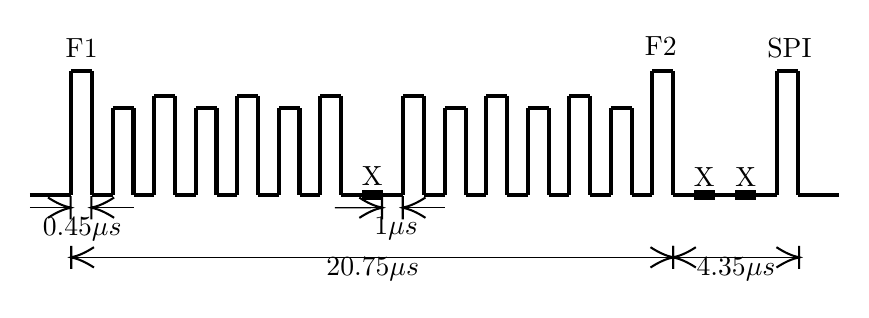
\begin{tikzpicture}[x=0.75pt,y=0.75pt,yscale=-1,xscale=1]
%uncomment if require: \path (0,180.203125); %set diagram left start at 0, and has height of 180.203125

%Straight Lines [id:da802619575601567]
\draw [line width=1.5]    (20,94.04) -- (40,94.04) ;


%Straight Lines [id:da8846665583581863]
\draw [line width=1.5]    (70,94.04) -- (80,94.04) ;


%Straight Lines [id:da3547989817438646]
\draw [line width=1.5]    (80,46.16) -- (80,94.04) ;


%Straight Lines [id:da6786393993290907]
\draw [line width=1.5]    (90,46.16) -- (90,94.04) ;


%Straight Lines [id:da12112819050786516]
\draw [line width=1.5]    (80,46.16) -- (90,46.16) ;



%Straight Lines [id:da07255526125264633]
\draw [line width=1.5]    (100,52.15) -- (100,94.04) ;


%Straight Lines [id:da05627008980696768]
\draw [line width=1.5]    (110,52.15) -- (110,94.04) ;


%Straight Lines [id:da9730765698164527]
\draw [line width=1.5]    (100,52.15) -- (110,52.15) ;



%Straight Lines [id:da6228472555399085]
\draw [line width=1.5]    (90,94.04) -- (100,94.04) ;


%Straight Lines [id:da4417024657143669]
\draw [line width=1.5]    (120,46.16) -- (120,94.04) ;


%Straight Lines [id:da6201546778263647]
\draw [line width=1.5]    (130,46.16) -- (130,94.04) ;


%Straight Lines [id:da28201313684151197]
\draw [line width=1.5]    (120,46.16) -- (130,46.16) ;



%Straight Lines [id:da6361182126863407]
\draw [line width=1.5]    (110,94.04) -- (120,94.04) ;


%Straight Lines [id:da6747728824147963]
\draw [line width=1.5]    (130,94.04) -- (140,94.04) ;


%Straight Lines [id:da3224432090670297]
\draw [line width=1.5]    (140,52.15) -- (140,94.04) ;


%Straight Lines [id:da3459996283003486]
\draw [line width=1.5]    (150,52.15) -- (150,94.04) ;


%Straight Lines [id:da20825687017459593]
\draw [line width=1.5]    (140,52.15) -- (150,52.15) ;



%Straight Lines [id:da17008537769438514]
\draw [line width=1.5]    (150,94.04) -- (160,94.04) ;


%Straight Lines [id:da6430642161538729]
\draw [line width=1.5]    (160,46.16) -- (160,94.04) ;


%Straight Lines [id:da9910395905777125]
\draw [line width=1.5]    (170,46.16) -- (170,94.04) ;


%Straight Lines [id:da8815258408442321]
\draw [line width=1.5]    (160,46.16) -- (170,46.16) ;



%Straight Lines [id:da48153782916369203]
\draw [line width=1.5]    (230,94.04) -- (240,94.04) ;


%Straight Lines [id:da6152359779178163]
\draw [line width=1.5]    (210,94.04) -- (220,94.04) ;


%Straight Lines [id:da9576750050734197]
\draw [line width=1.5]    (190,94.04) -- (200,94.04) ;


%Straight Lines [id:da5894247879142442]
\draw [line width=1.5]    (170,94.04) -- (180,94.04) ;


%Straight Lines [id:da5938221264909751]
\draw [line width=1.5]    (200,46.16) -- (200,94.04) ;


%Straight Lines [id:da535898962515496]
\draw [line width=1.5]    (210,46.16) -- (210,94.04) ;


%Straight Lines [id:da3330921253393093]
\draw [line width=1.5]    (200,46.16) -- (210,46.16) ;



%Straight Lines [id:da3197332364560672]
\draw [line width=3.75]    (180,94.04) -- (190,94.04) ;


%Straight Lines [id:da11643619546062678]
\draw [line width=1.5]    (290,94.04) -- (300,94.04) ;


%Straight Lines [id:da9122489192221612]
\draw [line width=1.5]    (270,94.04) -- (280,94.04) ;


%Straight Lines [id:da37951722352537964]
\draw [line width=1.5]    (250,94.04) -- (260,94.04) ;


%Straight Lines [id:da9469334675875289]
\draw [line width=1.5]    (220,52.15) -- (220,94.04) ;


%Straight Lines [id:da49406254585434173]
\draw [line width=1.5]    (230,52.15) -- (230,94.04) ;


%Straight Lines [id:da7118637832685069]
\draw [line width=1.5]    (220,52.15) -- (230,52.15) ;



%Straight Lines [id:da3101319760713177]
\draw [line width=1.5]    (240,46.16) -- (240,94.04) ;


%Straight Lines [id:da4027117306542707]
\draw [line width=1.5]    (250,46.16) -- (250,94.04) ;


%Straight Lines [id:da8543164668530872]
\draw [line width=1.5]    (240,46.16) -- (250,46.16) ;



%Straight Lines [id:da8462253053537638]
\draw [line width=1.5]    (260,52.15) -- (260,94.04) ;


%Straight Lines [id:da765419963120815]
\draw [line width=1.5]    (270,52.15) -- (270,94.04) ;


%Straight Lines [id:da4726948003847433]
\draw [line width=1.5]    (260,52.15) -- (270,52.15) ;



%Straight Lines [id:da6704242502929196]
\draw [line width=1.5]    (280,46.16) -- (280,94.04) ;


%Straight Lines [id:da22064815342513078]
\draw [line width=1.5]    (290,46.16) -- (290,94.04) ;


%Straight Lines [id:da4760105507577064]
\draw [line width=1.5]    (280,46.16) -- (290,46.16) ;



%Straight Lines [id:da9773349853639779]
\draw [line width=1.5]    (300,52.15) -- (300,94.04) ;


%Straight Lines [id:da2763151819570615]
\draw [line width=1.5]    (310,52.15) -- (310,94.04) ;


%Straight Lines [id:da7333450103165968]
\draw [line width=1.5]    (300,52.15) -- (310,52.15) ;



%Straight Lines [id:da451907340744798]
\draw [line width=1.5]    (60,52.15) -- (60,94.04) ;


%Straight Lines [id:da1265436924292953]
\draw [line width=1.5]    (70,52.15) -- (70,94.04) ;


%Straight Lines [id:da1660173504300022]
\draw [line width=1.5]    (60,52.15) -- (70,52.15) ;



%Straight Lines [id:da34960184621806967]
\draw [line width=1.5]    (40,34.19) -- (40,94.04) ;


%Straight Lines [id:da8463913463076289]
\draw [line width=1.5]    (50,34.19) -- (50,94.04) ;


%Straight Lines [id:da04867166916554311]
\draw [line width=1.5]    (40,34.19) -- (50,34.19) ;



%Straight Lines [id:da7032942910244449]
\draw [line width=1.5]    (50,94.04) -- (60,94.04) ;


%Straight Lines [id:da4906235653553823]
\draw [line width=1.5]    (310,94.04) -- (320,94.04) ;


%Straight Lines [id:da3046983205898657]
\draw [line width=1.5]    (330,94.04) -- (340,94.04) ;


%Straight Lines [id:da44493794365476447]
\draw [line width=1.5]    (320,34.19) -- (320,94.04) ;


%Straight Lines [id:da7873489358513719]
\draw [line width=1.5]    (330,34.19) -- (330,94.04) ;


%Straight Lines [id:da8719802383903079]
\draw [line width=1.5]    (320,34.19) -- (330,34.19) ;



%Straight Lines [id:da9818959957640496]
\draw [line width=1.5]    (390,94.04) -- (410,94.04) ;


%Straight Lines [id:da13121398375253968]
\draw [line width=1.5]    (380,34.19) -- (380,94.04) ;


%Straight Lines [id:da39388590475564844]
\draw [line width=1.5]    (390,34.19) -- (390,94.04) ;


%Straight Lines [id:da1556083423044594]
\draw [line width=1.5]    (380,34.19) -- (390,34.19) ;



%Straight Lines [id:da5428730812448004]
\draw [line width=3.75]    (340,94.04) -- (350,94.04) ;


%Straight Lines [id:da33723013140125846]
\draw [line width=1.5]    (350,94.04) -- (360,94.04) ;


%Straight Lines [id:da3223584265184558]
\draw [line width=3.75]    (360,94.04) -- (370,94.04) ;


%Straight Lines [id:da0016058567486934017]
\draw [line width=1.5]    (370,94.04) -- (380,94.04) ;


%Straight Lines [id:da03439474336491766]
\draw    (20,100.03) -- (39.72,100.03) ;
\draw [shift={(39.72,100.03)}, rotate = 180] [color={rgb, 255:red, 0; green, 0; blue, 0 }  ][line width=0.75]    (0,5.59) -- (0,-5.59)(10.93,-4.9) .. controls (6.95,-2.3) and (3.31,-0.67) .. (0,0) .. controls (3.31,0.67) and (6.95,2.3) .. (10.93,4.9)   ;

%Straight Lines [id:da8097926563979791]
\draw    (70,100.03) -- (49.72,100.03) ;
\draw [shift={(49.72,100.03)}, rotate = 360] [color={rgb, 255:red, 0; green, 0; blue, 0 }  ][line width=0.75]    (0,5.59) -- (0,-5.59)(10.93,-4.9) .. controls (6.95,-2.3) and (3.31,-0.67) .. (0,0) .. controls (3.31,0.67) and (6.95,2.3) .. (10.93,4.9)   ;

%Straight Lines [id:da01688783181234821]
\draw    (167,100.09) -- (189.72,100.03) ;
\draw [shift={(189.72,100.03)}, rotate = 539.8399999999999] [color={rgb, 255:red, 0; green, 0; blue, 0 }  ][line width=0.75]    (0,5.59) -- (0,-5.59)(10.93,-4.9) .. controls (6.95,-2.3) and (3.31,-0.67) .. (0,0) .. controls (3.31,0.67) and (6.95,2.3) .. (10.93,4.9)   ;

%Straight Lines [id:da5297584760495793]
\draw    (220,100.03) -- (199.72,100.03) ;
\draw [shift={(199.72,100.03)}, rotate = 360] [color={rgb, 255:red, 0; green, 0; blue, 0 }  ][line width=0.75]    (0,5.59) -- (0,-5.59)(10.93,-4.9) .. controls (6.95,-2.3) and (3.31,-0.67) .. (0,0) .. controls (3.31,0.67) and (6.95,2.3) .. (10.93,4.9)   ;

%Straight Lines [id:da3348624599545036]
\draw    (330,123.97) -- (40,123.97) ;
\draw [shift={(40,123.97)}, rotate = 360] [color={rgb, 255:red, 0; green, 0; blue, 0 }  ][line width=0.75]    (0,5.59) -- (0,-5.59)(10.93,-4.9) .. controls (6.95,-2.3) and (3.31,-0.67) .. (0,0) .. controls (3.31,0.67) and (6.95,2.3) .. (10.93,4.9)   ;
\draw [shift={(330,123.97)}, rotate = 180] [color={rgb, 255:red, 0; green, 0; blue, 0 }  ][line width=0.75]    (0,5.59) -- (0,-5.59)(10.93,-4.9) .. controls (6.95,-2.3) and (3.31,-0.67) .. (0,0) .. controls (3.31,0.67) and (6.95,2.3) .. (10.93,4.9)   ;
%Straight Lines [id:da7312758116993645]
\draw    (330,123.97) -- (390.69,123.97) ;
\draw [shift={(390.69,123.97)}, rotate = 180] [color={rgb, 255:red, 0; green, 0; blue, 0 }  ][line width=0.75]    (0,5.59) -- (0,-5.59)(10.93,-4.9) .. controls (6.95,-2.3) and (3.31,-0.67) .. (0,0) .. controls (3.31,0.67) and (6.95,2.3) .. (10.93,4.9)   ;
\draw [shift={(330,123.97)}, rotate = 0] [color={rgb, 255:red, 0; green, 0; blue, 0 }  ][line width=0.75]    (0,5.59) -- (0,-5.59)(10.93,-4.9) .. controls (6.95,-2.3) and (3.31,-0.67) .. (0,0) .. controls (3.31,0.67) and (6.95,2.3) .. (10.93,4.9)   ;

% Text Node
\draw (45,23.31) node  [align=left] {F1};
% Text Node
\draw (324,22.31) node  [align=left] {F2};
% Text Node
\draw (386,23.31) node  [align=left] {SPI};
% Text Node
\draw (185,84.56) node  [align=left] {X};
% Text Node
\draw (345,85.16) node  [align=left] {X};
% Text Node
\draw (365,85.16) node  [align=left] {X};
% Text Node
\draw (47.5,110.5) node  [align=left] {0.45$\displaystyle \mu s$ };
% Text Node
\draw (198.72,109.9) node  [align=left] {1$\displaystyle \mu s$ };
% Text Node
\draw (187.5,129.65) node  [align=left] {20.75$\displaystyle \mu s$ };
% Text Node
\draw (362.5,129.65) node  [align=left] {4.35$\displaystyle \mu s$ };


\end{tikzpicture}

  }
  \caption{Mode~A/C interrogation pulses}
  \label{fig:mode_ac_downlink_pulses}
\end{figure}

The response type (A or C) cannot be identified based on the reply signal itself. The SSR determines the content based on the synchronization with interrogations. This design of ATCRBS works sufficiently well with low-density air traffic, but it cannot efficiently cope with higher flight densities. Since all aircraft replies are transmitted on the same frequency, when several aircraft are in the same direction of the radar beam, reply signals can overlap and introduce errors for decoding. This is known as synchronous garbling.

When there are multiply secondary radars in the vicinity, replies originated by other radars may be considered as valid responses of one radar, which in turn, causes errors and confusion. This syndrome is called FRUIT (False Replies Unsynchronized In Time).

Though some of the garbling and the FRUIT problem can be mitigated with the reduction of interrogation frequency and improvements in signal processing ability, the information transmitted in Mode~A and Mode~C is still very limited. The number of identity codes available in Mode~A communication is limited to a maximum of 4096 unique codes, which poses another clear limitation.

Hence, more advanced communication protocols needed to be developed to acquire more information from a large number of aircraft.



\section{Mode~S}

Mode~S (Mode~Select Beacon System) was designed by Lincoln Laboratory at Massachusetts Institute of Technology in the 1970s. Based on different iterations of hardware and software design in the 1980s, the implementation of Mode~S in air traffic control began in the 1990s. Since then, Mode~S has become one of the main sources for aircraft surveillance.

The main characteristic of Mode~S is its selective interrogation, which allows the SSR to interrogate different information from different aircraft separately. By using selective interrogation, it largely mitigated the problem of garbling in Mode~A/C and thus greatly improved the capacity of the communication channel.

Unlike the limited number (4096) of unique identification codes in Mode~A communication, the Mode~S transponder is identified by a 24-bit transponder code, which can support up to 16,777,216 ($2^{24}$) unique addresses. In addition to these two major advantages, the Mode~S protocol introduced many different types of information that could be interrogated and downlinked.

\subsection{Mode~S interrogations}
The Mode~S uplink signal contains parameters that indicate which information is desired by the air traffic controller. There are two types of Mode~S interrogations, which are shown in Figure \ref{fig:mode_s_uplink_pulses}. The short interrogation has 56 bits of information contained in the data block, while the long interrogation contains 112 bits of information. The P2 pulse acts as the sidelobe suppression for Mode~A/C transponders so that they will ignore the rest of the interrogation pulses. Information in the Mode~S interrogation data block is uses the Differential Phase-Shift Keying (DPSK) modulaion \cite{mazda2014}.

\begin{figure}[ht]
  \scalebox{0.9}{
    

\tikzset{every picture/.style={line width=0.75pt}} %set default line width to 0.75pt

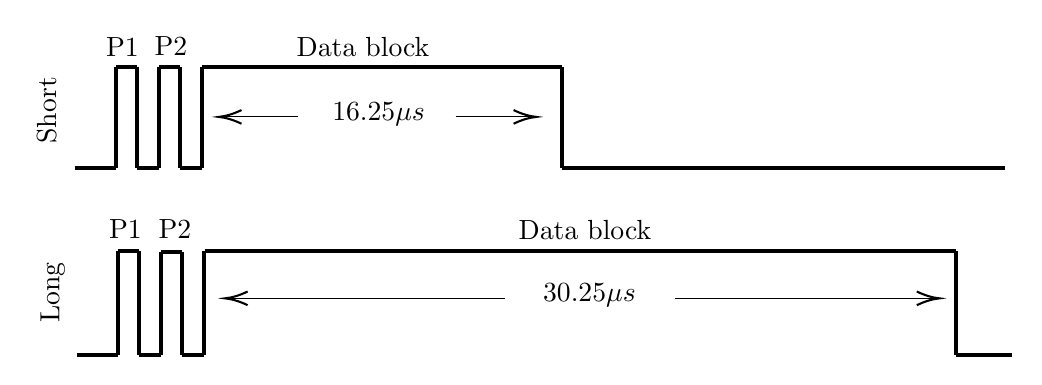
\begin{tikzpicture}[x=0.75pt,y=0.75pt,yscale=-1,xscale=1]
%uncomment if require: \path (0,217.796875); %set diagram left start at 0, and has height of 217.796875

%Straight Lines [id:da5463474554890266]
\draw [line width=1.5]    (36.74,81.1) -- (56.55,81.1) ;


%Straight Lines [id:da011025260001845005]
\draw [line width=1.5]    (56.55,32.59) -- (56.55,81.1) ;


%Straight Lines [id:da9700915149156659]
\draw [line width=1.5]    (66.45,81.1) -- (77.34,81.1) ;


%Straight Lines [id:da7292614282159362]
\draw [line width=1.5]    (66.45,32.59) -- (66.45,81.1) ;


%Straight Lines [id:da2120636052839573]
\draw [line width=1.5]    (56.55,32.59) -- (66.45,32.59) ;


%Straight Lines [id:da7407727471329684]
\draw [line width=1.5]    (77.34,32.66) -- (77.34,81.1) ;


%Straight Lines [id:da3086315118284293]
\draw [line width=1.5]    (87.24,32.66) -- (87.24,81.1) ;


%Straight Lines [id:da43471856317955515]
\draw [line width=1.5]    (77.34,32.66) -- (87.24,32.66) ;


%Straight Lines [id:da21748043219681268]
\draw [line width=1.5]    (271.3,81.1) -- (484.79,81.1) ;


%Straight Lines [id:da8605418823011517]
\draw [line width=1.5]    (98.13,32.59) -- (98.13,81.1) ;


%Straight Lines [id:da33837577584025946]
\draw [line width=1.5]    (271.3,32.59) -- (271.3,81.1) ;


%Straight Lines [id:da7189622162225036]
\draw [line width=1.5]    (98.13,32.59) -- (271.3,32.59) ;


%Straight Lines [id:da12987349167309414]
\draw [line width=1.5]    (87.24,81.1) -- (98.13,81.1) ;


%Straight Lines [id:da16740950379174557]
\draw    (220.1,56.61) -- (257,56.61) ;
\draw [shift={(259,56.61)}, rotate = 180] [color={rgb, 255:red, 0; green, 0; blue, 0 }  ][line width=0.75]    (10.93,-3.29) .. controls (6.95,-1.4) and (3.31,-0.3) .. (0,0) .. controls (3.31,0.3) and (6.95,1.4) .. (10.93,3.29)   ;

%Straight Lines [id:da9223288185776453]
\draw    (144.4,56.61) -- (108.04,56.61) ;
\draw [shift={(106.04,56.61)}, rotate = 360] [color={rgb, 255:red, 0; green, 0; blue, 0 }  ][line width=0.75]    (10.93,-3.29) .. controls (6.95,-1.4) and (3.31,-0.3) .. (0,0) .. controls (3.31,0.3) and (6.95,1.4) .. (10.93,3.29)   ;

%Straight Lines [id:da5604715690671425]
\draw [line width=1.5]    (37.7,171.23) -- (57.5,171.23) ;


%Straight Lines [id:da3482985767996405]
\draw [line width=1.5]    (57.5,121.24) -- (57.5,171.23) ;


%Straight Lines [id:da4509700113624615]
\draw [line width=1.5]    (67.4,171.23) -- (78.29,171.23) ;


%Straight Lines [id:da6288824727066149]
\draw [line width=1.5]    (67.4,121.24) -- (67.4,171.23) ;


%Straight Lines [id:da9575214566084325]
\draw [line width=1.5]    (57.5,121.24) -- (67.4,121.24) ;


%Straight Lines [id:da6700340501722795]
\draw [line width=1.5]    (78.29,121.66) -- (78.29,171.23) ;


%Straight Lines [id:da4549188813303331]
\draw [line width=1.5]    (88.19,121.66) -- (88.19,171.23) ;


%Straight Lines [id:da13620972501671025]
\draw [line width=1.5]    (78.29,121.66) -- (88.19,121.66) ;


%Straight Lines [id:da8658134392734089]
\draw [line width=1.5]    (461.31,171.23) -- (488,171.23) ;


%Straight Lines [id:da5147728308566684]
\draw [line width=1.5]    (99.08,121.24) -- (99.08,171.23) ;


%Straight Lines [id:da36847889433801817]
\draw [line width=1.5]    (461.31,121.24) -- (461.31,171.23) ;


%Straight Lines [id:da25047917548281684]
\draw [line width=1.5]    (99.19,121.24) -- (461.31,121.24) ;


%Straight Lines [id:da2857122828422307]
\draw [line width=1.5]    (88.19,171.23) -- (99.08,171.23) ;


%Straight Lines [id:da06287647464295643]
\draw    (326,144.03) -- (451.28,144.03) ;
\draw [shift={(453.28,144.03)}, rotate = 180] [color={rgb, 255:red, 0; green, 0; blue, 0 }  ][line width=0.75]    (10.93,-3.29) .. controls (6.95,-1.4) and (3.31,-0.3) .. (0,0) .. controls (3.31,0.3) and (6.95,1.4) .. (10.93,3.29)   ;

%Straight Lines [id:da5064106996156972]
\draw    (244,144.03) -- (111,144.03) ;
\draw [shift={(109,144.03)}, rotate = 360] [color={rgb, 255:red, 0; green, 0; blue, 0 }  ][line width=0.75]    (10.93,-3.29) .. controls (6.95,-1.4) and (3.31,-0.3) .. (0,0) .. controls (3.31,0.3) and (6.95,1.4) .. (10.93,3.29)   ;


% Text Node
\draw (59.6,23.12) node  [align=left] {P1};
% Text Node
\draw (82.95,22.69) node  [align=left] {P2};
% Text Node
\draw (175.52,22.69) node  [align=left] {Data block};
% Text Node
\draw (185.25,55.47) node  [align=left] {16.25$\displaystyle \mu s$ };
% Text Node
\draw (61.07,110.58) node  [align=left] {P1};
% Text Node
\draw (84.9,110.53) node  [align=left] {P2};
% Text Node
\draw (282.45,111.04) node  [align=left] {Data block};
% Text Node
\draw (286.85,142.62) node  [align=left] {30.25$\displaystyle \mu s$ };
% Text Node
\draw (23.03,53.44) node [rotate=-270] [align=left] {Short};
% Text Node
\draw (26.03,141.19) node [rotate=-270] [align=left] {Long};


\end{tikzpicture}

  }
  \caption{Mode~S uplink pulses}
  \label{fig:mode_s_uplink_pulses}
\end{figure}


\subsection{Mode~S replies}
There two types of Mode~S downlink signals, short reply and long reply, which correspond to the short and long interrogations from the SSR. For each microsecond, two bits are transmitted. All Mode~S replies start with an 8-microsecond fixed preamble and continue with 56 or 122 microseconds of the data block. The structure of the downlink message is shown in Figure \ref{fig:mode_s_downlink_pulses}.

\begin{figure}[ht]
  \scalebox{0.9}{
    

\tikzset{every picture/.style={line width=0.75pt}} %set default line width to 0.75pt

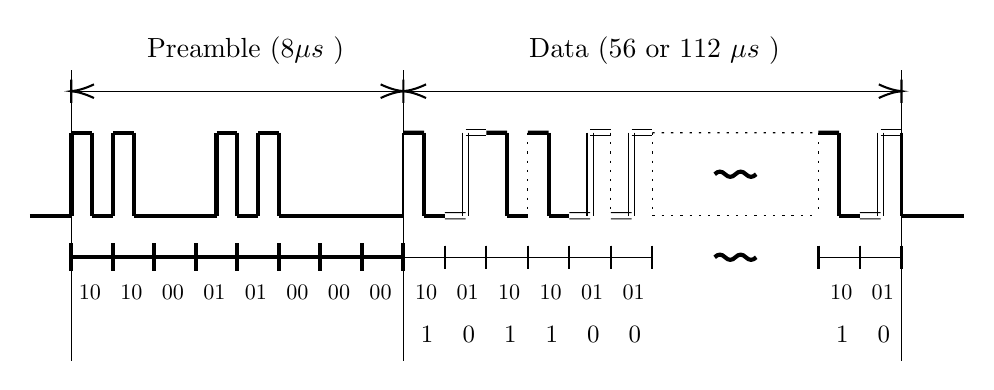
\begin{tikzpicture}[x=0.75pt,y=0.75pt,yscale=-1,xscale=1]
%uncomment if require: \path (0,300); %set diagram left start at 0, and has height of 300

%Straight Lines [id:da19456008639159283]
\draw [line width=1.5]    (50,140) -- (70.1,140) ;


%Straight Lines [id:da4966520337198381]
\draw [line width=1.5]    (70.1,100.01) -- (70.1,140) ;


%Straight Lines [id:da17227664765792117]
\draw [line width=1.5]    (80.05,100.01) -- (80.05,140) ;


%Straight Lines [id:da33186369020888096]
\draw [line width=1.5]    (70.1,100.01) -- (80.05,100.01) ;


%Straight Lines [id:da5988664999522268]
\draw [line width=1.5]    (470,140) -- (500,140) ;


%Straight Lines [id:da9277065502847237]
\draw [line width=0.75]    (230,100.01) -- (230,140) ;


%Straight Lines [id:da9681563991623432]
\draw [line width=0.75]    (470,100) -- (470,140) ;


%Straight Lines [id:da7098007092204757]
\draw    (232,80) -- (470,80) ;
\draw [shift={(470,80)}, rotate = 180] [color={rgb, 255:red, 0; green, 0; blue, 0 }  ][line width=0.75]    (0,5.59) -- (0,-5.59)(10.93,-3.29) .. controls (6.95,-1.4) and (3.31,-0.3) .. (0,0) .. controls (3.31,0.3) and (6.95,1.4) .. (10.93,3.29)   ;
\draw [shift={(230,80)}, rotate = 0] [color={rgb, 255:red, 0; green, 0; blue, 0 }  ][line width=0.75]    (10.93,-3.29) .. controls (6.95,-1.4) and (3.31,-0.3) .. (0,0) .. controls (3.31,0.3) and (6.95,1.4) .. (10.93,3.29)   ;
%Straight Lines [id:da006227256180845631]
\draw [line width=1.5]    (80.05,140) -- (90.16,140) ;


%Straight Lines [id:da6036579810043201]
\draw [line width=1.5]    (90.16,100.01) -- (90.16,140) ;


%Straight Lines [id:da00281388855623832]
\draw [line width=1.5]    (100.1,100.01) -- (100.1,140) ;


%Straight Lines [id:da31107781342094976]
\draw [line width=1.5]    (90.16,100.01) -- (100.1,100.01) ;


%Straight Lines [id:da7535133896366635]
\draw [line width=1.5]    (100.1,140) -- (140,140) ;


%Straight Lines [id:da12899924992549905]
\draw [line width=1.5]    (140,100.01) -- (140,140) ;


%Straight Lines [id:da5378098501650792]
\draw [line width=1.5]    (149.95,100.01) -- (149.95,140) ;


%Straight Lines [id:da20360679771004464]
\draw [line width=1.5]    (140,100.01) -- (149.95,100.01) ;


%Straight Lines [id:da0662339058123167]
\draw [line width=1.5]    (160,100.01) -- (160,140) ;


%Straight Lines [id:da4007151351628726]
\draw [line width=1.5]    (169.95,100.01) -- (169.95,140) ;


%Straight Lines [id:da8355934189325502]
\draw [line width=1.5]    (160,100.01) -- (169.95,100.01) ;


%Straight Lines [id:da3384414628493404]
\draw [line width=1.5]    (149.95,140) -- (160,140) ;


%Straight Lines [id:da16959694459003116]
\draw [line width=1.5]    (169.95,140) -- (230,140) ;


%Straight Lines [id:da6341834757656402]
\draw    (70,80) -- (230,80) ;
\draw [shift={(230,80)}, rotate = 180] [color={rgb, 255:red, 0; green, 0; blue, 0 }  ][line width=0.75]    (0,5.59) -- (0,-5.59)(10.93,-3.29) .. controls (6.95,-1.4) and (3.31,-0.3) .. (0,0) .. controls (3.31,0.3) and (6.95,1.4) .. (10.93,3.29)   ;
\draw [shift={(70,80)}, rotate = 0] [color={rgb, 255:red, 0; green, 0; blue, 0 }  ][line width=0.75]    (0,5.59) -- (0,-5.59)(10.93,-3.29) .. controls (6.95,-1.4) and (3.31,-0.3) .. (0,0) .. controls (3.31,0.3) and (6.95,1.4) .. (10.93,3.29)   ;
%Straight Lines [id:da0823697857509611]
\draw [line width=1.5]    (240,100) -- (240,140) ;


%Straight Lines [id:da5965240827324876]
\draw [line width=1.5]    (230,100.01) -- (240,100) ;


%Straight Lines [id:da5388260517365404]
\draw [line width=1.5]    (240,140) -- (250,140) ;


%Straight Lines [id:da8600091413630995]
\draw    (261.5,100) -- (261.5,140)(258.5,100) -- (258.5,140) ;


%Straight Lines [id:da27698119200143934]
\draw    (250,138.5) -- (260,138.49)(250,141.5) -- (260,141.49) ;


%Straight Lines [id:da10856086064332326]
\draw    (260,98.5) -- (270,98.5)(260,101.5) -- (270,101.5) ;


%Straight Lines [id:da005734725357589898]
\draw [line width=1.5]    (280,100) -- (280,140) ;


%Straight Lines [id:da5978065202252392]
\draw [line width=1.5]    (270,100.01) -- (280,100) ;


%Straight Lines [id:da4952820421686712]
\draw [line width=1.5]    (280,140) -- (290,140) ;


%Straight Lines [id:da8758683524376032]
\draw [line width=1.5]    (300,100) -- (300,140) ;


%Straight Lines [id:da1174267939792284]
\draw [line width=1.5]    (290,100.01) -- (300,100) ;


%Straight Lines [id:da5508059799734031]
\draw [line width=1.5]    (300,140) -- (310,140) ;


%Straight Lines [id:da5916201151331775]
\draw  [dash pattern={on 0.84pt off 2.51pt}]  (290,100) -- (290,140) ;


%Straight Lines [id:da09623948592314746]
\draw    (230,160) -- (250,160) ;
\draw [shift={(250,160)}, rotate = 180] [color={rgb, 255:red, 0; green, 0; blue, 0 }  ][line width=0.75]    (0,5.59) -- (0,-5.59)   ;
\draw [shift={(230,160)}, rotate = 180] [color={rgb, 255:red, 0; green, 0; blue, 0 }  ][line width=0.75]    (0,5.59) -- (0,-5.59)   ;
%Straight Lines [id:da793930081283176]
\draw    (250,160) -- (270,160) ;
\draw [shift={(270,160)}, rotate = 180] [color={rgb, 255:red, 0; green, 0; blue, 0 }  ][line width=0.75]    (0,5.59) -- (0,-5.59)   ;
\draw [shift={(250,160)}, rotate = 180] [color={rgb, 255:red, 0; green, 0; blue, 0 }  ][line width=0.75]    (0,5.59) -- (0,-5.59)   ;
%Straight Lines [id:da6912169606656351]
\draw    (270,160) -- (290,160) ;
\draw [shift={(290,160)}, rotate = 180] [color={rgb, 255:red, 0; green, 0; blue, 0 }  ][line width=0.75]    (0,5.59) -- (0,-5.59)   ;
\draw [shift={(270,160)}, rotate = 180] [color={rgb, 255:red, 0; green, 0; blue, 0 }  ][line width=0.75]    (0,5.59) -- (0,-5.59)   ;
%Straight Lines [id:da7289875132082819]
\draw    (290,160) -- (310,160) ;
\draw [shift={(310,160)}, rotate = 180] [color={rgb, 255:red, 0; green, 0; blue, 0 }  ][line width=0.75]    (0,5.59) -- (0,-5.59)   ;
\draw [shift={(290,160)}, rotate = 180] [color={rgb, 255:red, 0; green, 0; blue, 0 }  ][line width=0.75]    (0,5.59) -- (0,-5.59)   ;
%Straight Lines [id:da08758041142379525]
\draw    (321.5,100) -- (321.5,140)(318.5,100) -- (318.5,140) ;


%Straight Lines [id:da045381193792315866]
\draw    (310,138.5) -- (320,138.49)(310,141.5) -- (320,141.49) ;


%Straight Lines [id:da17135944504759926]
\draw    (320,98.5) -- (330,98.5)(320,101.5) -- (330,101.5) ;


%Straight Lines [id:da17944423145609467]
\draw    (341.5,100) -- (341.5,140)(338.5,100) -- (338.5,140) ;


%Straight Lines [id:da7713063525502672]
\draw    (330,138.5) -- (340,138.49)(330,141.5) -- (340,141.49) ;


%Straight Lines [id:da33146902749837825]
\draw    (340,98.5) -- (350,98.5)(340,101.5) -- (350,101.5) ;


%Straight Lines [id:da9879355240362433]
\draw  [dash pattern={on 0.84pt off 2.51pt}]  (330,100) -- (330,140) ;


%Straight Lines [id:da036051775482985216]
\draw    (310,160) -- (330,160) ;
\draw [shift={(330,160)}, rotate = 180] [color={rgb, 255:red, 0; green, 0; blue, 0 }  ][line width=0.75]    (0,5.59) -- (0,-5.59)   ;
\draw [shift={(310,160)}, rotate = 180] [color={rgb, 255:red, 0; green, 0; blue, 0 }  ][line width=0.75]    (0,5.59) -- (0,-5.59)   ;
%Straight Lines [id:da28859620775073025]
\draw    (330,160) -- (350,160) ;
\draw [shift={(350,160)}, rotate = 180] [color={rgb, 255:red, 0; green, 0; blue, 0 }  ][line width=0.75]    (0,5.59) -- (0,-5.59)   ;
\draw [shift={(330,160)}, rotate = 180] [color={rgb, 255:red, 0; green, 0; blue, 0 }  ][line width=0.75]    (0,5.59) -- (0,-5.59)   ;
%Straight Lines [id:da16671927493599492]
\draw [line width=1.5]    (380,120) .. controls (381.67,118.33) and (383.33,118.33) .. (385,120) .. controls (386.67,121.67) and (388.33,121.67) .. (390,120) .. controls (391.67,118.33) and (393.33,118.33) .. (395,120) .. controls (396.67,121.67) and (398.33,121.67) .. (400,120) -- (400,120) ;


%Straight Lines [id:da8138130724046564]
\draw [line width=1.5]    (440,100) -- (440,140) ;


%Straight Lines [id:da22958393404437416]
\draw [line width=1.5]    (430,100.01) -- (440,100) ;


%Straight Lines [id:da9881209239338602]
\draw [line width=1.5]    (440,140) -- (450,140) ;


%Straight Lines [id:da8083425801534385]
\draw    (461.5,100) -- (461.5,140)(458.5,100) -- (458.5,140) ;


%Straight Lines [id:da5168655767549837]
\draw    (450,138.5) -- (460,138.49)(450,141.5) -- (460,141.49) ;


%Straight Lines [id:da9334334900115471]
\draw    (460,98.5) -- (470,98.5)(460,101.5) -- (470,101.5) ;


%Straight Lines [id:da7737429504279858]
\draw    (430,160) -- (450,160) ;
\draw [shift={(450,160)}, rotate = 180] [color={rgb, 255:red, 0; green, 0; blue, 0 }  ][line width=0.75]    (0,5.59) -- (0,-5.59)   ;
\draw [shift={(430,160)}, rotate = 180] [color={rgb, 255:red, 0; green, 0; blue, 0 }  ][line width=0.75]    (0,5.59) -- (0,-5.59)   ;
%Straight Lines [id:da83916450948631]
\draw    (450,160) -- (470,160) ;
\draw [shift={(470,160)}, rotate = 180] [color={rgb, 255:red, 0; green, 0; blue, 0 }  ][line width=0.75]    (0,5.59) -- (0,-5.59)   ;
\draw [shift={(450,160)}, rotate = 180] [color={rgb, 255:red, 0; green, 0; blue, 0 }  ][line width=0.75]    (0,5.59) -- (0,-5.59)   ;
%Straight Lines [id:da550938742895299]
\draw [line width=1.5]    (380,160) .. controls (381.67,158.33) and (383.33,158.33) .. (385,160) .. controls (386.67,161.67) and (388.33,161.67) .. (390,160) .. controls (391.67,158.33) and (393.33,158.33) .. (395,160) .. controls (396.67,161.67) and (398.33,161.67) .. (400,160) -- (400,160) ;


%Straight Lines [id:da7040603522240081]
\draw  [dash pattern={on 0.84pt off 2.51pt}]  (350,100) -- (430,100.01) ;


%Straight Lines [id:da47067895049383823]
\draw  [dash pattern={on 0.84pt off 2.51pt}]  (350,140) -- (430,140) ;


%Straight Lines [id:da7869758290201998]
\draw  [dash pattern={on 0.84pt off 2.51pt}]  (350,100) -- (350,140) ;


%Straight Lines [id:da008409540135993376]
\draw  [dash pattern={on 0.84pt off 2.51pt}]  (430,100.01) -- (430,140.01) ;


%Straight Lines [id:da31788159730743515]
\draw [line width=1.5]    (70,160) -- (90,160) ;
\draw [shift={(90,160)}, rotate = 180] [color={rgb, 255:red, 0; green, 0; blue, 0 }  ][line width=1.5]    (0,6.71) -- (0,-6.71)   ;
\draw [shift={(70,160)}, rotate = 180] [color={rgb, 255:red, 0; green, 0; blue, 0 }  ][line width=1.5]    (0,6.71) -- (0,-6.71)   ;
%Straight Lines [id:da3106745365256183]
\draw [line width=1.5]    (90,160) -- (110,160) ;
\draw [shift={(110,160)}, rotate = 180] [color={rgb, 255:red, 0; green, 0; blue, 0 }  ][line width=1.5]    (0,6.71) -- (0,-6.71)   ;
\draw [shift={(90,160)}, rotate = 180] [color={rgb, 255:red, 0; green, 0; blue, 0 }  ][line width=1.5]    (0,6.71) -- (0,-6.71)   ;
%Straight Lines [id:da9907265074982001]
\draw [line width=1.5]    (110,160) -- (130,160) ;
\draw [shift={(130,160)}, rotate = 180] [color={rgb, 255:red, 0; green, 0; blue, 0 }  ][line width=1.5]    (0,6.71) -- (0,-6.71)   ;
\draw [shift={(110,160)}, rotate = 180] [color={rgb, 255:red, 0; green, 0; blue, 0 }  ][line width=1.5]    (0,6.71) -- (0,-6.71)   ;
%Straight Lines [id:da26596309543070085]
\draw [line width=1.5]    (130,160) -- (150,160) ;
\draw [shift={(150,160)}, rotate = 180] [color={rgb, 255:red, 0; green, 0; blue, 0 }  ][line width=1.5]    (0,6.71) -- (0,-6.71)   ;
\draw [shift={(130,160)}, rotate = 180] [color={rgb, 255:red, 0; green, 0; blue, 0 }  ][line width=1.5]    (0,6.71) -- (0,-6.71)   ;
%Straight Lines [id:da6888158581086454]
\draw [line width=1.5]    (150,160) -- (170,160) ;
\draw [shift={(170,160)}, rotate = 180] [color={rgb, 255:red, 0; green, 0; blue, 0 }  ][line width=1.5]    (0,6.71) -- (0,-6.71)   ;
\draw [shift={(150,160)}, rotate = 180] [color={rgb, 255:red, 0; green, 0; blue, 0 }  ][line width=1.5]    (0,6.71) -- (0,-6.71)   ;
%Straight Lines [id:da2905018729448581]
\draw [line width=1.5]    (170,160) -- (190,160) ;
\draw [shift={(190,160)}, rotate = 180] [color={rgb, 255:red, 0; green, 0; blue, 0 }  ][line width=1.5]    (0,6.71) -- (0,-6.71)   ;
\draw [shift={(170,160)}, rotate = 180] [color={rgb, 255:red, 0; green, 0; blue, 0 }  ][line width=1.5]    (0,6.71) -- (0,-6.71)   ;
%Straight Lines [id:da4484545554397412]
\draw [line width=1.5]    (190,160) -- (210,160) ;
\draw [shift={(210,160)}, rotate = 180] [color={rgb, 255:red, 0; green, 0; blue, 0 }  ][line width=1.5]    (0,6.71) -- (0,-6.71)   ;
\draw [shift={(190,160)}, rotate = 180] [color={rgb, 255:red, 0; green, 0; blue, 0 }  ][line width=1.5]    (0,6.71) -- (0,-6.71)   ;
%Straight Lines [id:da8423657346900506]
\draw [line width=1.5]    (210,160) -- (230,160) ;
\draw [shift={(230,160)}, rotate = 180] [color={rgb, 255:red, 0; green, 0; blue, 0 }  ][line width=1.5]    (0,6.71) -- (0,-6.71)   ;
\draw [shift={(210,160)}, rotate = 180] [color={rgb, 255:red, 0; green, 0; blue, 0 }  ][line width=1.5]    (0,6.71) -- (0,-6.71)   ;
%Straight Lines [id:da23665455383450085]
\draw    (230,70) -- (230,210) ;


%Straight Lines [id:da29641650098315697]
\draw    (70.1,70) -- (70.1,210) ;


%Straight Lines [id:da8192252165632716]
\draw    (470,70) -- (470,210) ;



% Text Node
\draw (154,60.5) node  [align=left] {Preamble (8$\displaystyle \mu s$ )};
% Text Node
\draw (351,60.5) node  [align=left] {Data (56 or 112 $\displaystyle \mu s$ )};
% Text Node
\draw (241,177) node [scale=0.8] [align=left] {10};
% Text Node
\draw (261,177) node [scale=0.8] [align=left] {01};
% Text Node
\draw (281,177) node [scale=0.8] [align=left] {10};
% Text Node
\draw (301,177) node [scale=0.8] [align=left] {10};
% Text Node
\draw (321,177) node [scale=0.8] [align=left] {01};
% Text Node
\draw (341,177) node [scale=0.8] [align=left] {01};
% Text Node
\draw (441,177) node [scale=0.8] [align=left] {10};
% Text Node
\draw (461,177) node [scale=0.8] [align=left] {01};
% Text Node
\draw (241.5,197) node [scale=0.9] [align=left] {1};
% Text Node
\draw (261.5,197) node [scale=0.9] [align=left] {0};
% Text Node
\draw (281.5,197) node [scale=0.9] [align=left] {1};
% Text Node
\draw (301.5,197) node [scale=0.9] [align=left] {1};
% Text Node
\draw (321.5,197) node [scale=0.9] [align=left] {0};
% Text Node
\draw (341.5,197) node [scale=0.9] [align=left] {0};
% Text Node
\draw (441.5,197) node [scale=0.9] [align=left] {1};
% Text Node
\draw (461.5,197) node [scale=0.9] [align=left] {0};
% Text Node
\draw (79,177) node [scale=0.8] [align=left] {10};
% Text Node
\draw (99,177) node [scale=0.8] [align=left] {10};
% Text Node
\draw (119,177) node [scale=0.8] [align=left] {00};
% Text Node
\draw (139,177) node [scale=0.8] [align=left] {01};
% Text Node
\draw (159,177) node [scale=0.8] [align=left] {01};
% Text Node
\draw (179,177) node [scale=0.8] [align=left] {00};
% Text Node
\draw (199,177) node [scale=0.8] [align=left] {00};
% Text Node
\draw (219,177) node [scale=0.8] [align=left] {00};


\end{tikzpicture}

  }
  \caption{An example of Mode~S reply message}
  \label{fig:mode_s_downlink_pulses}
\end{figure}

The 16-bit fix preamble can be represented as \texttt{1010000101000000} in binary. The information contained in the data block is modulated using the Pulse Position Modulation (PPM), which is a type of amplitude modulation. In PPM, the \1 bit is represented by a 0.5-microsecond of pulse followed by a 0.5-microsecond flat signal. The \0 bit is reversed compared to the \1 bit. It is represented by a 0.5-microsecond flat signal and followed by a 0.5-microsecond pulse.

\begin{notebox}{Note}
  Mode~S uplink and downlink signals use different modulation methods. The uplink uses phase modulation, while the downlink uses amplitude modulation. Phase modulation requires slightly more complicated hardware implementation but has a better performance in terms of error tolerance. 
\end{notebox}

\subsection{Compatiblity with Mode~A/C}

Similar to Mode~A/C, Mode~S SSR can send \emph{All-Call} interrogations to all aircraft in the vicinity. The All-Call interrogations are designed to be compatible with Mode~A/C transponders. In Figure \ref{fig:mode_s_all_call}, the All-Call interrogation is shown. There would be 8 or 21 microseconds between P1 and P3, which is the same as Mode~A/C. P4 is a wider pulse lasting for 1.6 microseconds.

\begin{figure}[ht]
  \scalebox{0.9}{
    

\tikzset{every picture/.style={line width=0.75pt}} %set default line width to 0.75pt

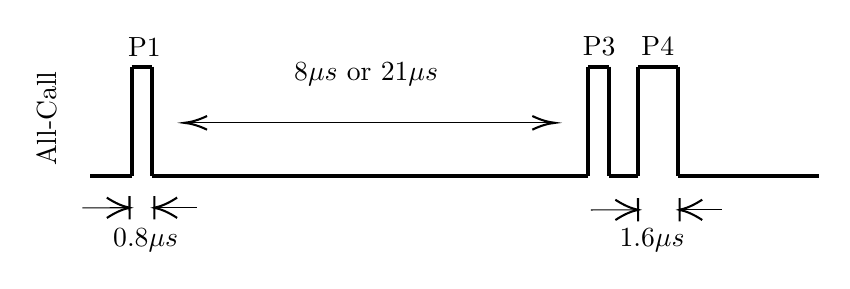
\begin{tikzpicture}[x=0.75pt,y=0.75pt,yscale=-1,xscale=1]
%uncomment if require: \path (0,195.52841186523438); %set diagram left start at 0, and has height of 195.52841186523438

%Straight Lines [id:da6908913326121413]
\draw [line width=1.5]    (48.72,89.58) -- (68.72,89.58) ;


%Straight Lines [id:da7314812061278786]
\draw [line width=1.5]    (68.72,36.79) -- (68.72,89.58) ;


%Straight Lines [id:da8295464365532541]
\draw [line width=1.5]    (78.72,89.58) -- (288.72,89.58) ;


%Straight Lines [id:da8762398433428527]
\draw [line width=1.5]    (78.72,36.79) -- (78.72,89.58) ;


%Straight Lines [id:da6322670680533355]
\draw [line width=1.5]    (68.72,36.79) -- (78.72,36.79) ;


%Straight Lines [id:da9574535991728885]
\draw [line width=1.5]    (288.72,36.79) -- (288.72,89.58) ;


%Straight Lines [id:da32386192110336776]
\draw [line width=1.5]    (298.72,36.79) -- (298.72,89.58) ;


%Straight Lines [id:da3992451139630393]
\draw [line width=1.5]    (288.72,36.79) -- (298.72,36.79) ;


%Straight Lines [id:da059171585354682144]
\draw [line width=1.5]    (298.72,89.58) -- (312.72,89.58) ;


%Straight Lines [id:da8536188761146808]
\draw    (96.14,63.85) -- (270.72,63.85) ;
\draw [shift={(272.72,63.85)}, rotate = 180] [color={rgb, 255:red, 0; green, 0; blue, 0 }  ][line width=0.75]    (10.93,-3.29) .. controls (6.95,-1.4) and (3.31,-0.3) .. (0,0) .. controls (3.31,0.3) and (6.95,1.4) .. (10.93,3.29)   ;
\draw [shift={(94.14,63.85)}, rotate = 0] [color={rgb, 255:red, 0; green, 0; blue, 0 }  ][line width=0.75]    (10.93,-3.29) .. controls (6.95,-1.4) and (3.31,-0.3) .. (0,0) .. controls (3.31,0.3) and (6.95,1.4) .. (10.93,3.29)   ;
%Straight Lines [id:da6322642144532382]
\draw    (45,104.82) -- (67.72,104.76) ;
\draw [shift={(67.72,104.76)}, rotate = 539.85] [color={rgb, 255:red, 0; green, 0; blue, 0 }  ][line width=0.75]    (0,5.59) -- (0,-5.59)(10.93,-4.9) .. controls (6.95,-2.3) and (3.31,-0.67) .. (0,0) .. controls (3.31,0.67) and (6.95,2.3) .. (10.93,4.9)   ;

%Straight Lines [id:da15280489267069064]
\draw    (100,104.76) -- (79.72,104.76) ;
\draw [shift={(79.72,104.76)}, rotate = 360] [color={rgb, 255:red, 0; green, 0; blue, 0 }  ][line width=0.75]    (0,5.59) -- (0,-5.59)(10.93,-4.9) .. controls (6.95,-2.3) and (3.31,-0.67) .. (0,0) .. controls (3.31,0.67) and (6.95,2.3) .. (10.93,4.9)   ;

%Straight Lines [id:da350935368675795]
\draw [line width=1.5]    (312.72,36.79) -- (312.72,89.58) ;


%Straight Lines [id:da4852523934905475]
\draw [line width=1.5]    (331.84,36.79) -- (331.84,89.58) ;


%Straight Lines [id:da2665349700634352]
\draw [line width=1.5]    (312.72,36.79) -- (331.84,36.79) ;


%Straight Lines [id:da45062356526910285]
\draw [line width=1.5]    (331.84,89.58) -- (400.14,89.58) ;


%Straight Lines [id:da0013962966443246128]
\draw    (290,105.82) -- (312.72,105.76) ;
\draw [shift={(312.72,105.76)}, rotate = 539.85] [color={rgb, 255:red, 0; green, 0; blue, 0 }  ][line width=0.75]    (0,5.59) -- (0,-5.59)(10.93,-4.9) .. controls (6.95,-2.3) and (3.31,-0.67) .. (0,0) .. controls (3.31,0.67) and (6.95,2.3) .. (10.93,4.9)   ;

%Straight Lines [id:da16918775558415122]
\draw    (353,105.76) -- (332.72,105.76) ;
\draw [shift={(332.72,105.76)}, rotate = 360] [color={rgb, 255:red, 0; green, 0; blue, 0 }  ][line width=0.75]    (0,5.59) -- (0,-5.59)(10.93,-4.9) .. controls (6.95,-2.3) and (3.31,-0.67) .. (0,0) .. controls (3.31,0.67) and (6.95,2.3) .. (10.93,4.9)   ;


% Text Node
\draw (74.89,27.54) node  [align=left] {P1};
% Text Node
\draw (294,27) node  [align=left] {P3};
% Text Node
\draw (181.72,40.56) node  [align=left] {8$\displaystyle \mu s$ or 21$\displaystyle \mu s$};
% Text Node
\draw (27.72,61.85) node [rotate=-270] [align=left] {All-Call};
% Text Node
\draw (77.72,120.33) node  [align=left] {0.8$\displaystyle \mu s$ };
% Text Node
\draw (322.23,27) node  [align=left] {P4};
% Text Node
\draw (321.72,120.33) node  [align=left] {1.6$\displaystyle \mu s$ };


\end{tikzpicture}

  }
  \caption{Mode~A/C/S All-Call interrogation}
  \label{fig:mode_s_all_call}
\end{figure}

When a Mode~A/C transponder receives this interrogation, the last pulse P4 is ignored. Hence, a normal Mode~A or Mode~C reply is replied. A Mode~S transponder would detect P4, and thus, produce a Mode~S All-Call reply. The Mode~A/C/S All-Call reply is designed for SSR to identify which aircraft are in the vicinity, including Mode~A/C only aircraft.

This is one of the several different interrogation pulse patterns from a Mode~A/C compatible Mode~S radar. Most current SSRs can perform both Mode~A/C and Mode~S interrogations. In Figure \ref{fig:mode_s_inter_mode}, the interrogation pulses and replies from aircraft transponders are summarized.

\begin{figure}[ht]
  \scalebox{0.9}{
    

% Pattern Info
 
\tikzset{
pattern size/.store in=\mcSize, 
pattern size = 5pt,
pattern thickness/.store in=\mcThickness, 
pattern thickness = 0.3pt,
pattern radius/.store in=\mcRadius, 
pattern radius = 1pt}
\makeatletter
\pgfutil@ifundefined{pgf@pattern@name@_xbfmcxt9a}{
\pgfdeclarepatternformonly[\mcThickness,\mcSize]{_xbfmcxt9a}
{\pgfqpoint{0pt}{0pt}}
{\pgfpoint{\mcSize}{\mcSize}}
{\pgfpoint{\mcSize}{\mcSize}}
{
\pgfsetcolor{\tikz@pattern@color}
\pgfsetlinewidth{\mcThickness}
\pgfpathmoveto{\pgfqpoint{0pt}{\mcSize}}
\pgfpathlineto{\pgfpoint{\mcSize+\mcThickness}{-\mcThickness}}
\pgfpathmoveto{\pgfqpoint{0pt}{0pt}}
\pgfpathlineto{\pgfpoint{\mcSize+\mcThickness}{\mcSize+\mcThickness}}
\pgfusepath{stroke}
}}
\makeatother

% Pattern Info
 
\tikzset{
pattern size/.store in=\mcSize, 
pattern size = 5pt,
pattern thickness/.store in=\mcThickness, 
pattern thickness = 0.3pt,
pattern radius/.store in=\mcRadius, 
pattern radius = 1pt}
\makeatletter
\pgfutil@ifundefined{pgf@pattern@name@_xk0qj1gra}{
\pgfdeclarepatternformonly[\mcThickness,\mcSize]{_xk0qj1gra}
{\pgfqpoint{0pt}{0pt}}
{\pgfpoint{\mcSize}{\mcSize}}
{\pgfpoint{\mcSize}{\mcSize}}
{
\pgfsetcolor{\tikz@pattern@color}
\pgfsetlinewidth{\mcThickness}
\pgfpathmoveto{\pgfqpoint{0pt}{\mcSize}}
\pgfpathlineto{\pgfpoint{\mcSize+\mcThickness}{-\mcThickness}}
\pgfpathmoveto{\pgfqpoint{0pt}{0pt}}
\pgfpathlineto{\pgfpoint{\mcSize+\mcThickness}{\mcSize+\mcThickness}}
\pgfusepath{stroke}
}}
\makeatother

% Pattern Info
 
\tikzset{
pattern size/.store in=\mcSize, 
pattern size = 5pt,
pattern thickness/.store in=\mcThickness, 
pattern thickness = 0.3pt,
pattern radius/.store in=\mcRadius, 
pattern radius = 1pt}
\makeatletter
\pgfutil@ifundefined{pgf@pattern@name@_2pgsvssh0}{
\pgfdeclarepatternformonly[\mcThickness,\mcSize]{_2pgsvssh0}
{\pgfqpoint{0pt}{0pt}}
{\pgfpoint{\mcSize}{\mcSize}}
{\pgfpoint{\mcSize}{\mcSize}}
{
\pgfsetcolor{\tikz@pattern@color}
\pgfsetlinewidth{\mcThickness}
\pgfpathmoveto{\pgfqpoint{0pt}{\mcSize}}
\pgfpathlineto{\pgfpoint{\mcSize+\mcThickness}{-\mcThickness}}
\pgfpathmoveto{\pgfqpoint{0pt}{0pt}}
\pgfpathlineto{\pgfpoint{\mcSize+\mcThickness}{\mcSize+\mcThickness}}
\pgfusepath{stroke}
}}
\makeatother
\tikzset{every picture/.style={line width=0.75pt}} %set default line width to 0.75pt        

\begin{tikzpicture}[x=0.75pt,y=0.75pt,yscale=-1,xscale=1]
%uncomment if require: \path (0,420); %set diagram left start at 0, and has height of 420

%Straight Lines [id:da10139563460007883] 
\draw [line width=1.5]    (13.62,106.11) -- (26.7,106.11) ;
%Straight Lines [id:da8944987457679359] 
\draw [line width=1.5]    (26.7,71.61) -- (26.7,106.11) ;
%Straight Lines [id:da8726787727488281] 
\draw [line width=1.5]    (33.24,106.11) -- (170.55,106.11) ;
%Straight Lines [id:da23155927698345424] 
\draw [line width=1.5]    (33.24,71.61) -- (33.24,106.11) ;
%Straight Lines [id:da6621871356145643] 
\draw [line width=1.5]    (26.7,71.61) -- (33.24,71.61) ;
%Straight Lines [id:da8244081669931158] 
\draw [line width=1.5]    (170.55,71.61) -- (170.55,106.11) ;
%Straight Lines [id:da7952592463602781] 
\draw [line width=1.5]    (177.09,71.61) -- (177.09,106.11) ;
%Straight Lines [id:da41254632967840155] 
\draw [line width=1.5]    (170.55,71.61) -- (177.09,71.61) ;
%Straight Lines [id:da9690069379761994] 
\draw [line width=1.5]    (177.09,106.11) -- (283.04,106.11) ;
%Straight Lines [id:da15712603919924883] 
\draw    (133.42,87.78) -- (159.42,87.78) ;
\draw [shift={(161.42,87.78)}, rotate = 180] [color={rgb, 255:red, 0; green, 0; blue, 0 }  ][line width=0.75]    (10.93,-3.29) .. controls (6.95,-1.4) and (3.31,-0.3) .. (0,0) .. controls (3.31,0.3) and (6.95,1.4) .. (10.93,3.29)   ;
%Straight Lines [id:da8177870286653945] 
\draw    (68.42,87.78) -- (43.01,87.78) ;
\draw [shift={(41.01,87.78)}, rotate = 360] [color={rgb, 255:red, 0; green, 0; blue, 0 }  ][line width=0.75]    (10.93,-3.29) .. controls (6.95,-1.4) and (3.31,-0.3) .. (0,0) .. controls (3.31,0.3) and (6.95,1.4) .. (10.93,3.29)   ;
%Straight Lines [id:da4130868707940596] 
\draw [line width=1.5]    (13.31,178.54) -- (26.39,178.54) ;
%Straight Lines [id:da6104484319886425] 
\draw [line width=1.5]    (26.39,142.87) -- (26.39,178.54) ;
%Straight Lines [id:da729839123466383] 
\draw [line width=1.5]    (32.93,178.54) -- (170.24,178.54) ;
%Straight Lines [id:da46210972259749217] 
\draw [line width=1.5]    (32.93,142.87) -- (32.93,178.54) ;
%Straight Lines [id:da3946646049493354] 
\draw [line width=1.5]    (26.39,142.87) -- (32.93,142.87) ;
%Straight Lines [id:da45361249491466893] 
\draw [line width=1.5]    (170.24,142.87) -- (170.24,178.54) ;
%Straight Lines [id:da013066896381340287] 
\draw [line width=1.5]    (176.78,142.87) -- (176.78,178.54) ;
%Straight Lines [id:da5125811046438047] 
\draw [line width=1.5]    (170.24,142.87) -- (176.78,142.87) ;
%Straight Lines [id:da04670638385217374] 
\draw [line width=1.5]    (191.68,178.54) -- (282.81,178.54) ;
%Straight Lines [id:da6527055724791548] 
\draw    (136.42,158.44) -- (159.51,158.44) ;
\draw [shift={(161.51,158.44)}, rotate = 180] [color={rgb, 255:red, 0; green, 0; blue, 0 }  ][line width=0.75]    (10.93,-3.29) .. controls (6.95,-1.4) and (3.31,-0.3) .. (0,0) .. controls (3.31,0.3) and (6.95,1.4) .. (10.93,3.29)   ;
%Straight Lines [id:da36183606845289473] 
\draw    (69.42,158.44) -- (43.35,158.44) ;
\draw [shift={(41.35,158.44)}, rotate = 360] [color={rgb, 255:red, 0; green, 0; blue, 0 }  ][line width=0.75]    (10.93,-3.29) .. controls (6.95,-1.4) and (3.31,-0.3) .. (0,0) .. controls (3.31,0.3) and (6.95,1.4) .. (10.93,3.29)   ;
%Straight Lines [id:da6505599521554695] 
\draw [line width=1.5]    (184.63,142.87) -- (184.63,178.54) ;
%Straight Lines [id:da8362755930589003] 
\draw [line width=1.5]    (191.68,142.87) -- (191.68,178.54) ;
%Straight Lines [id:da9657378828407124] 
\draw [line width=1.5]    (184.63,142.87) -- (191.68,142.87) ;
%Straight Lines [id:da07819410086631895] 
\draw [line width=1.5]    (176.78,178.54) -- (184.63,178.54) ;
%Straight Lines [id:da42606907148767026] 
\draw [line width=1.5]    (12.7,332.08) -- (25.77,332.08) ;
%Straight Lines [id:da9369974037547926] 
\draw [line width=1.5]    (25.77,295.12) -- (25.77,332.08) ;
%Straight Lines [id:da33291206879252355] 
\draw [line width=1.5]    (32.31,332.08) -- (39.5,332.08) ;
%Straight Lines [id:da5240912720550126] 
\draw [line width=1.5]    (32.31,295.12) -- (32.31,332.08) ;
%Straight Lines [id:da9330494691664342] 
\draw [line width=1.5]    (25.77,295.12) -- (32.31,295.12) ;
%Straight Lines [id:da8890541249124149] 
\draw [line width=1.5]    (39.5,295.12) -- (39.5,332.08) ;
%Straight Lines [id:da4307963117279683] 
\draw [line width=1.5]    (46.04,295.12) -- (46.04,332.08) ;
%Straight Lines [id:da9617422203980213] 
\draw [line width=1.5]    (39.5,295.12) -- (46.04,295.12) ;
%Straight Lines [id:da4479242464721258] 
\draw [line width=1.5]    (267.76,332.08) -- (283.58,332.08) ;
%Straight Lines [id:da6100425835249386] 
\draw [line width=1.5]    (53.24,295.12) -- (53.24,332.08) ;
%Straight Lines [id:da5622846341893553] 
\draw [line width=1.5]    (267.76,295.12) -- (267.76,332.08) ;
%Straight Lines [id:da5535575889222741] 
\draw [line width=1.5]    (53.24,295.12) -- (267.76,295.12) ;
%Straight Lines [id:da5205414923951106] 
\draw [line width=1.5]    (46.04,332.08) -- (53.24,332.08) ;
%Straight Lines [id:da5941488225614739] 
\draw    (221,313.38) -- (259.69,313.38) ;
\draw [shift={(261.69,313.38)}, rotate = 180] [color={rgb, 255:red, 0; green, 0; blue, 0 }  ][line width=0.75]    (10.93,-3.29) .. controls (6.95,-1.4) and (3.31,-0.3) .. (0,0) .. controls (3.31,0.3) and (6.95,1.4) .. (10.93,3.29)   ;
%Straight Lines [id:da6033888492668897] 
\draw    (101,313.38) -- (60.47,313.38) ;
\draw [shift={(58.47,313.38)}, rotate = 360] [color={rgb, 255:red, 0; green, 0; blue, 0 }  ][line width=0.75]    (10.93,-3.29) .. controls (6.95,-1.4) and (3.31,-0.3) .. (0,0) .. controls (3.31,0.3) and (6.95,1.4) .. (10.93,3.29)   ;
%Shape: Rectangle [id:dp3759569294112588] 
\draw  [color={rgb, 255:red, 170; green, 170; blue, 170 }  ,draw opacity=1 ][pattern=_xbfmcxt9a,pattern size=7.5pt,pattern thickness=0.75pt,pattern radius=0pt, pattern color={rgb, 255:red, 204; green, 204; blue, 204}][line width=1.5]  (395,63.66) -- (465,63.66) -- (465,103.66) -- (395,103.66) -- cycle ;
%Straight Lines [id:da567943888440936] 
\draw    (291.5,5.25) -- (291.5,344.75) ;
%Straight Lines [id:da43129766275376125] 
\draw    (383.5,5.5) -- (383.5,344.25) ;
%Shape: Rectangle [id:dp13650423213785512] 
\draw  [color={rgb, 255:red, 170; green, 170; blue, 170 }  ,draw opacity=1 ][pattern=_xk0qj1gra,pattern size=7.5pt,pattern thickness=0.75pt,pattern radius=0pt, pattern color={rgb, 255:red, 204; green, 204; blue, 204}][line width=1.5]  (301,286.66) -- (372.5,286.66) -- (372.5,326.66) -- (301,326.66) -- cycle ;
%Straight Lines [id:da4022947807372834] 
\draw [line width=1.5]    (13.31,252.54) -- (26.39,252.54) ;
%Straight Lines [id:da3513929993035185] 
\draw [line width=1.5]    (26.39,216.87) -- (26.39,252.54) ;
%Straight Lines [id:da19278300475351973] 
\draw [line width=1.5]    (32.93,252.54) -- (170.24,252.54) ;
%Straight Lines [id:da7070427973197562] 
\draw [line width=1.5]    (32.93,216.87) -- (32.93,252.54) ;
%Straight Lines [id:da7452912603363431] 
\draw [line width=1.5]    (26.39,216.87) -- (32.93,216.87) ;
%Straight Lines [id:da23036923315310087] 
\draw [line width=1.5]    (170.24,216.87) -- (170.24,252.54) ;
%Straight Lines [id:da8834681986348356] 
\draw [line width=1.5]    (176.78,216.87) -- (176.78,252.54) ;
%Straight Lines [id:da6090727165571825] 
\draw [line width=1.5]    (170.24,216.87) -- (176.78,216.87) ;
%Straight Lines [id:da583647242134385] 
\draw [line width=1.5]    (198.18,252.54) -- (282.81,252.54) ;
%Straight Lines [id:da9170789589416013] 
\draw    (136.42,232.44) -- (159.51,232.44) ;
\draw [shift={(161.51,232.44)}, rotate = 180] [color={rgb, 255:red, 0; green, 0; blue, 0 }  ][line width=0.75]    (10.93,-3.29) .. controls (6.95,-1.4) and (3.31,-0.3) .. (0,0) .. controls (3.31,0.3) and (6.95,1.4) .. (10.93,3.29)   ;
%Straight Lines [id:da5167018156114838] 
\draw    (69.42,232.44) -- (43.35,232.44) ;
\draw [shift={(41.35,232.44)}, rotate = 360] [color={rgb, 255:red, 0; green, 0; blue, 0 }  ][line width=0.75]    (10.93,-3.29) .. controls (6.95,-1.4) and (3.31,-0.3) .. (0,0) .. controls (3.31,0.3) and (6.95,1.4) .. (10.93,3.29)   ;
%Straight Lines [id:da8566907298865956] 
\draw [line width=1.5]    (184.63,216.87) -- (184.63,252.54) ;
%Straight Lines [id:da7203690891559582] 
\draw [line width=1.5]    (198.18,216.87) -- (198.18,252.54) ;
%Straight Lines [id:da94538242427855] 
\draw [line width=1.5]    (184.63,216.87) -- (198.18,216.87) ;
%Straight Lines [id:da4235130725536582] 
\draw [line width=1.5]    (176.78,252.54) -- (184.63,252.54) ;
%Shape: Rectangle [id:dp11689677188470982] 
\draw  [color={rgb, 255:red, 170; green, 170; blue, 170 }  ,draw opacity=1 ][pattern=_2pgsvssh0,pattern size=7.5pt,pattern thickness=0.75pt,pattern radius=0pt, pattern color={rgb, 255:red, 204; green, 204; blue, 204}][line width=1.5]  (395,136.16) -- (465,136.16) -- (465,176.16) -- (395,176.16) -- cycle ;
%Straight Lines [id:da6780360984439984] 
\draw    (4,119.75) -- (477.5,119.75) ;
%Straight Lines [id:da13657082545459254] 
\draw    (4,192.75) -- (477.5,192.75) ;
%Straight Lines [id:da9967862276250885] 
\draw    (4,267.75) -- (477.5,267.75) ;
%Shape: Rectangle [id:dp8062164155653335] 
\draw   (4,5.25) -- (477.5,5.25) -- (477.5,343.75) -- (4,343.75) -- cycle ;
%Straight Lines [id:da6528849896631663] 
\draw    (4,49.75) -- (477.5,49.75) ;

% Text Node
\draw (30.73,62.45) node  [font=\small] [align=left] {P1};
% Text Node
\draw (174.47,63.03) node  [font=\small] [align=left] {P3};
% Text Node
\draw (103.2,87.59) node  [font=\small] [align=left] {8 / 21$\displaystyle \mu s$ };
% Text Node
\draw (103.55,158.26) node  [font=\small] [align=left] {8 / 21$\displaystyle \mu s$ };
% Text Node
\draw (27.15,285.77) node  [font=\small] [align=left] {P1};
% Text Node
\draw (46.19,285.42) node  [font=\small] [align=left] {P2};
% Text Node
\draw (150.35,285.42) node  [font=\small] [align=left] {Data block};
% Text Node
\draw (162.09,313.8) node  [font=\small] [align=left] {16.25 / 30.25$\displaystyle \mu s$ };
% Text Node
\draw (337.5,28.45) node  [font=\small] [align=left] {Mode A/C\\Transponder};
% Text Node
\draw (429.5,28.45) node  [font=\small] [align=left] {Mode S\\Transponder};
% Text Node
\draw  [line width=1.5]   (304.5,63.4) -- (371.5,63.4) -- (371.5,103.4) -- (304.5,103.4) -- cycle  ;
\draw (338,83.4) node  [font=\small] [align=left] {Mode A/C\\Reply};
% Text Node
\draw (430,83.66) node  [font=\small] [align=left] {Ignore};
% Text Node
\draw  [line width=1.5]   (397,286.82) -- (463,286.82) -- (463,326.82) -- (397,326.82) -- cycle  ;
\draw (430,306.82) node  [font=\small] [align=left] {Mode S \ \ \\Reply};
% Text Node
\draw  [line width=1.5]   (303.5,136.47) -- (370.5,136.47) -- (370.5,176.47) -- (303.5,176.47) -- cycle  ;
\draw (337,156.47) node  [font=\small] [align=left] {Mode A/C\\Reply};
% Text Node
\draw (79.47,28.45) node [anchor=west] [inner sep=0.75pt]  [font=\small] [align=left] {SSR Interrogations};
% Text Node
\draw (30.73,133.91) node  [font=\small] [align=left] {P1};
% Text Node
\draw (171.47,133.74) node  [font=\small] [align=left] {P3};
% Text Node
\draw (192.47,133.74) node  [font=\small] [align=left] {P4};
% Text Node
\draw (336.75,306.66) node  [font=\small] [align=left] {Ignore};
% Text Node
\draw (103.55,232.26) node  [font=\small] [align=left] {8 / 21$\displaystyle \mu s$ };
% Text Node
\draw  [line width=1.5]   (397,210.73) -- (463,210.73) -- (463,250.73) -- (397,250.73) -- cycle  ;
\draw (430,230.73) node  [font=\small] [align=left] {All-Call \ \ \ \\Reply};
% Text Node
\draw  [line width=1.5]   (303.5,210.47) -- (370.5,210.47) -- (370.5,250.47) -- (303.5,250.47) -- cycle  ;
\draw (337,230.47) node  [font=\small] [align=left] {Mode A/C\\Reply};
% Text Node
\draw (30.73,207.91) node  [font=\small] [align=left] {P1};
% Text Node
\draw (172.47,207.74) node  [font=\small] [align=left] {P3};
% Text Node
\draw (194.47,207.74) node  [font=\small] [align=left] {P4};
% Text Node
\draw (430,156.16) node  [font=\small] [align=left] {Ignore};
% Text Node
\draw (282.98,149.5) node [anchor=east] [inner sep=0.75pt]  [font=\scriptsize] [align=left] {\begin{minipage}[lt]{49.289392pt}\setlength\topsep{0pt}
\begin{flushright}
\textit{Mode A/C only}\\\textit{All-Call}
\end{flushright}

\end{minipage}};
% Text Node
\draw (280.72,222) node [anchor=east] [inner sep=0.75pt]  [font=\scriptsize] [align=left] {\begin{minipage}[lt]{40.948784pt}\setlength\topsep{0pt}
\begin{flushright}
\textit{Mode A/C/S}\\\textit{All-Call}
\end{flushright}

\end{minipage}};


\end{tikzpicture}
  }
  \caption{SSR interrogations pulses and transponder replies}
  \label{fig:mode_s_inter_mode}
\end{figure}

We can see that:

\begin{itemize}
  \item Mode~A/C transponders respond to all interrogations with P1 and P3.
  \item When P4 is not present or a shorter P4 is used (as shown in the first and second patterns), Mode~S transponders will ignore the interrogations.
  \item Mode~S transponders will produce an All-Call reply to interrogations with a long P4. This interrogation is used to acquire all aircraft with either Mode~A/C or Mode~S capability.
  \item Finally, all Mode~S interrogation is designed to be ignored by Mode~A/C transponders due to the presence of P2 (as shown in the last pattern), which is considered as a side lobe suppression mechanism for Mode~A/C transponders.
\end{itemize}


\begin{notebox}{Note}
  Mode~S SSR is also able to produce a Mode~S only All-Call interrogation using the standard Mode~S uplink (with uplink format 11).
\end{notebox}


\subsection{Mode~S format}

The Mode~S communication protocol is designed to handle different types of uplink and downlink message formats. The first 5 bits of the uplink or downlink message define the uplink format (UF) or downlink format (DF) number of the message. Based on the UF/DF number, different structures of the data block are defined. In Table \ref{tb:mode_s_formats}, all available Mode~S formats are shown. Currently, 11 Mode~S formats are being used. Numbers not in this table are reserved for future use.

\begin{table}[ht]
\centering
\footnotesize
\caption{Mode~S uplink and downlink formats}
\label{tb:mode_s_formats}
\begin{tabular}{|l|l|l|l|}
\hline
\textbf{UF/DF} & \textbf{Bits} & \textbf{Uplink type} & \textbf{Downlink type} \\ \hline\hline
0 & 56 & Short air-air surveillance (ACAS) & Short air-air surveillance (ACAS) \\ \hline
4 & 56 & Surveillance, altitude request & Surveillance, altitude reply \\ \hline
5 & 56 & Surveillance, identity request & Surveillance, identity reply \\ \hline
11 & 56 & Mode~S All-Call & All-Call reply \\ \hline
\hline
16 & 112 & Long air-air surveillance (ACAS) & Long air-air surveillance (ACAS) \\ \hline
17 & 112 & - & Extended squitter \\ \hline
18 & 112 & - & Extended squitter / non transponder \\ \hline
19 & 112 & - & Military extended squitter \\ \hline
20 & 112 & Comm-A, altitude request & Comm-B, altitude reply \\ \hline
21 & 112 & Comm-A, identity request & Comm-B, identity reply \\ \hline
24 & 112 & Comm-C (ELM) & Comm-D (ELM) \\ \hline
\end{tabular}
\end{table}


\begin{notebox}{Note}
  Format number 24 is an exception. It is identified using only the first two bits, which must be \texttt{11}. All following bits are used for encoding other information.
\end{notebox}


We can see that the short 56-bit data block is used to encode messages with format numbers from 0 to 11. Messages with format numbers above 16 are encoded with the long 112-bit data block. Among all uplink formats, UF 17, 18, and 19 are not used. This is because the corresponding downlink messages (extended squitter messages) are designed to be broadcast automatically without the need for SSR interrogations. 

One of the most common applications for the extended squitter is the Automatic Dependent Surveillance-Broadcast service, which is also commonly known as ADS-B.


\section{ADS-B}

Automatic Dependent Surveillance-Broadcast (ADS-B) is a surveillance technology designed to allow aircraft to broadcast their flight state periodically without the need for interrogation. The word \emph{automatic} refers to the fact that no inputs from controllers or pilots are required. The word \emph{dependent} indicates this technology depends on information from other onboard systems, such as air data systems and navigation systems.

Common aircraft state parameters included in ADS-B are position, altitude, and speed. The position is determined by Global Navigation Satellite Systems (GNSS). The velocity is derived from the GNSS position and the inertial measurement system. The altitude information includes both barometric altitude and GNSS altitude. The barometric altitude is provided by the air data system. In addition to these primary state parameters, ADS-B also allows other information to be broadcast, for example, aircraft call-sign, accuracy indicators, integrity indicators, and operational status.

Different types of ADS-B messages are identified by Type Codes. The structures of these messages are all defined in ICAO documents, such as in \cite{icao9871v1} and \cite{rtca2011mops}. In Part I of this book, we will explain how these different types of ADS-B messages can be decoded.

\begin{notebox}{Note}
Originally, there were three candidates to build ADS-B: Mode~S Extended Squitter, VHF Data Link - Mode~4 (VDL4)), and Universal Access Transceiver (UAT). Different specifications are designed for these frequency channels \cite{rtca2011mops, rtca2002uat}. However, the Mode~S extended squitter implementation of ADS-B is the most adopted one among all candidates. UAT is only partially implemented in some countries like the USA, while VDL4 did not go beyond the test phase.
\end{notebox}


\section{Other Mode~S services}

The most common data format number used in Mode~S for information downlink are 4, 5, 20, and 21. Format 4 and 5 are short messages designed to acquire aircraft altitude and identity (similar to Mode~A/C messages). Downlink messages with format 20 or 21, as known as Comm-B messages, contain other information desired by air traffic controllers, in addition to altitude and identity.

In theory, up to 255 different message types are supported by the Mode~S Comm-B. A new parameter, Comm-B Data Selector (BDS), is designed to identify which additional information is included in Mode~S messages. It functions similarly to the Type Code of ADS-B message. In practice, not all 255 BDS codes are defined or used. 

A subgroup of these codes is commonly interrogated by air traffic controllers. By combining different BDS codes into groups, several Mode~S services are defined. The two most used services are Mode~S Elementary Surveillance (ELS) and Mode~S Enhanced Surveillance (EHS) \cite{grappel2008}. For example, in the European airspace, aircraft above certain takeoff weight category are required to have these capabilities enabled.

The Mode~S Elementary Surveillance (ELS) consists of four BDS codes (10, 17, 20, and 30). It provides basic information such as Mode~S capabilities, identification (callsign), and ACAS resolution advisory, in addition to the altitude or identity (squawk code) information. 

The Mode~S Enhanced Surveillance consists of three BDS codes (40, 50, and 60). It provides much more additional information on aircraft states, such as selected altitudes, true airspeed, indicated airspeed, Mach number, bank angle, and turn rate.

In addition to the common ELS and EHS, the meteorological routine air report (MRAR), and the meteorological hazard report (MHR) are also interrogated in some controlled airspaces. These reports provide weather-related information such as wind and temperature that are measured by the aircraft sensors.


\section{Summary}

In Figure \ref{fig:mode_s_services}, all aforementioned Mode~S services and their relationships with Mode~S downlink formats are illustrated.

\begin{figure}[ht]
  \centering
  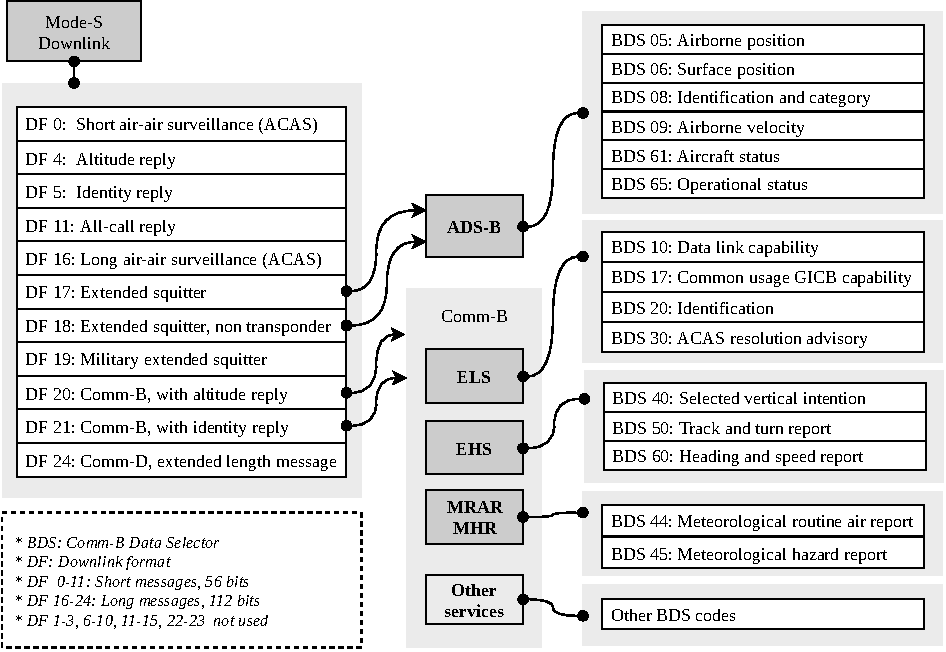
\includegraphics[width=\textwidth]{figures/intro/mode_s_services.pdf}
  \caption{Relationship between Mode~S downlink formats and different services}
  \label{fig:mode_s_services}
\end{figure}

In the rest of this book, the details of these services are discussed in different chapters. In chapter 2 (the rest of Part I), common hardware and software setups are shown. In chapter 3 to 10 (Part II), the focus is on ADS-B messages. Detailed guides on how to decode different types of messages are presented. In chapter 11 to 19 (Part III), the focus is on Mode~S ELS, EHS, and meteorological services. Accordingly, the decoding and inference of the messages are provided.
